\section{Употреба на приложението}
При стартиране на приложението се показва галерия с всички налични предмети, името и цената им. (Фиг. \ref{fig:home-screen-in-4})
\begin{figure}[H]
    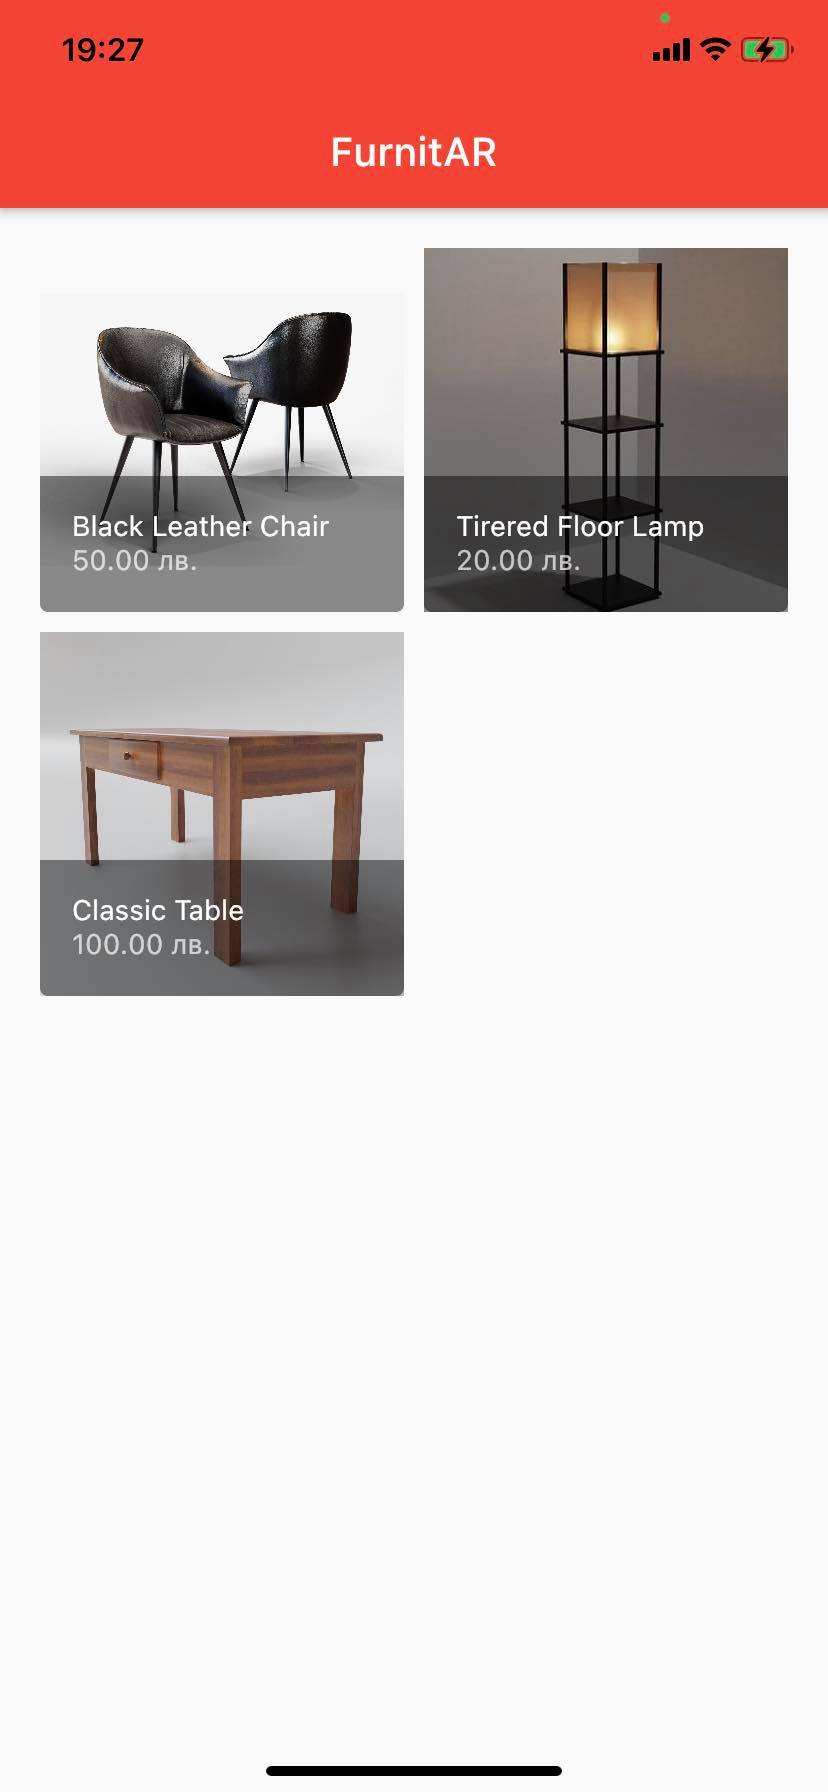
\includegraphics[width=0.5\textwidth]{home-screen-4.jpeg}
    \centering
    \caption{Начален екран на мобилното приложение}
    \label{fig:home-screen-in-4}
\end{figure}

От тази галерия може да се избере продукта, който да бъде визуализиран посредством аугментирана реалност. Преди избор от менюто, мобилното устройство трябва да се постави малко над мястото, където е желано да се проектира 3D модела на мебелта. След избор, камерата може да бъде преместена, като проекцията запазва положението си в пространството. (Фиг. \ref{fig:ar-screen-in-4})
\begin{figure}[H]
    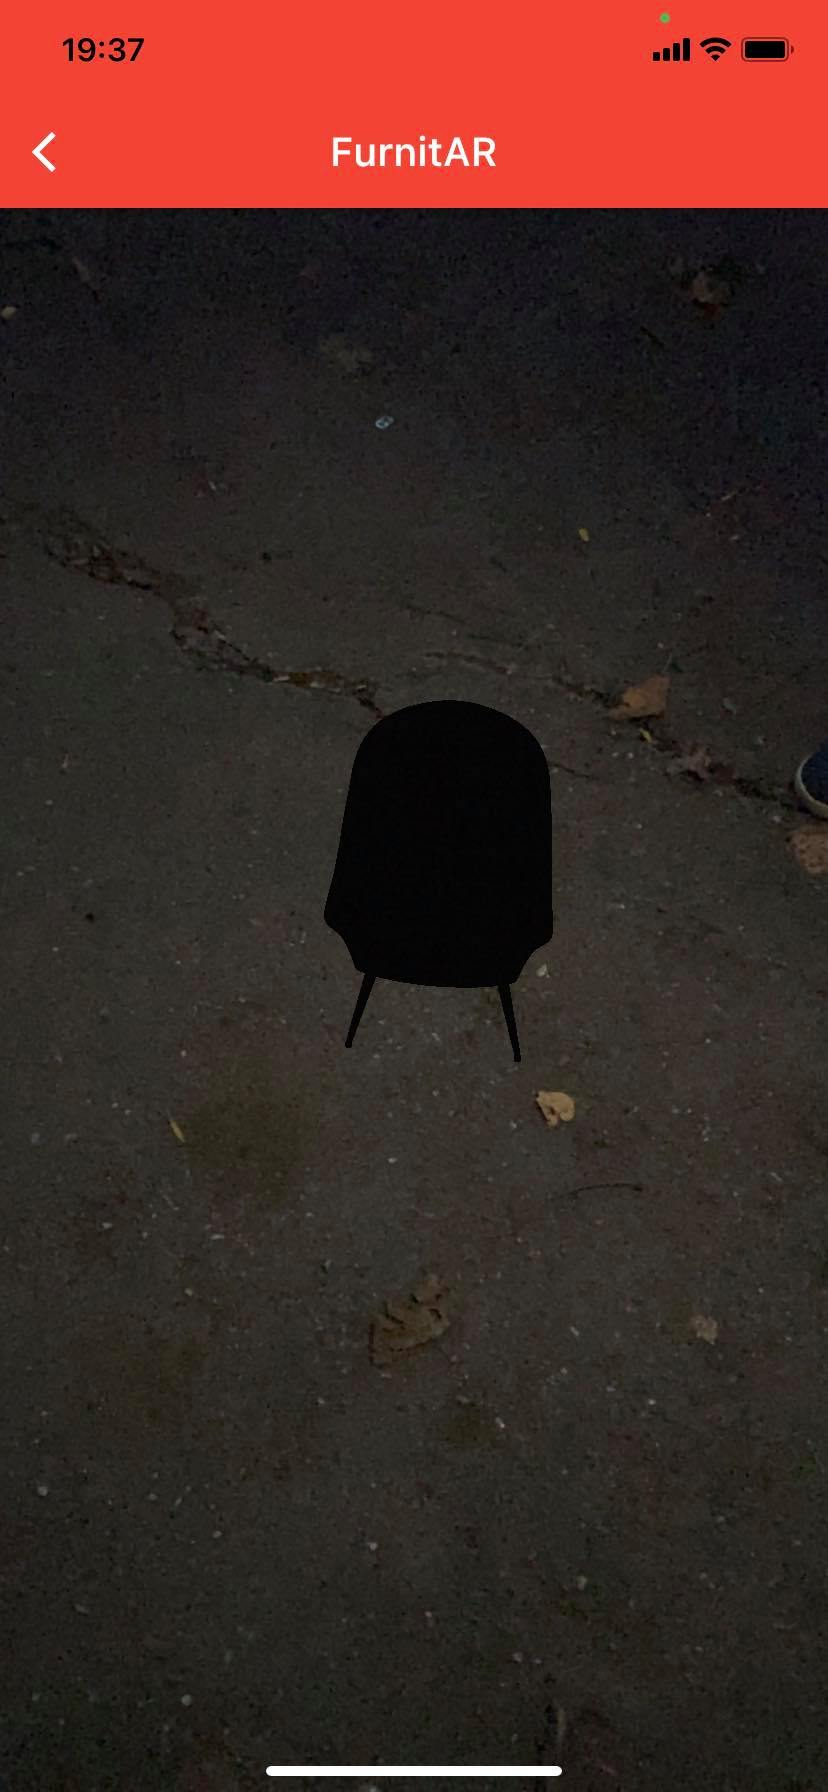
\includegraphics[width=0.5\textwidth]{ar-screen-4.jpeg}
    \centering
    \caption{AR визуализация в мобилното приложение}
    \label{fig:ar-screen-in-4}
\end{figure}